\documentclass[11pt,letterpaper,titlepage]{article}

%================== Document nomenclature
\newcommand{\DOCSUBJT}{ChiTech Whitepaper: }   %Put document subject here
\newcommand{\DOCTITLE}{                      %Put document title here
	Spherical Harmonics
}       
\newcommand{\DOCDATE} {August, 2018}         %Put document date here
\newcommand{\DOCREV}  {Rev 1.00}             %Put revision number here

%================== Misc Settings
\usepackage{fancyhdr}
\usepackage[left=0.75in, right=0.75in, bottom=1.0in]{geometry}
\usepackage{lastpage}
\usepackage{titleref}
\usepackage{booktabs}
\usepackage{appendix}

\appendixtitleon
\appendixtitletocon

\makeatletter

%================== List of figures and tables mods
\usepackage{tocloft}
\usepackage[labelfont=bf]{caption}

\renewcommand{\cftfigpresnum}{Figure\ }
\renewcommand{\cfttabpresnum}{Table\ }

\newlength{\mylenf}
\settowidth{\mylenf}{\cftfigpresnum}
\setlength{\cftfignumwidth}{\dimexpr\mylenf+3.5em}
\setlength{\cfttabnumwidth}{\dimexpr\mylenf+1.5em}



%=================== Graphics
\usepackage{graphicx}
\usepackage[breakwords]{truncate}
\usepackage{float}
\usepackage{array}
\usepackage{amsmath}
\usepackage{mdframed}
\usepackage{fancyvrb}
\usepackage{float}
\usepackage{cancel}
\usepackage{amssymb}
\graphicspath{ {images/} }
\usepackage[usenames,dvipsnames,svgnames,table]{xcolor}
\usepackage[defaultlines=2,all]{nowidow}
\usepackage{listings}
\usepackage{color}
\definecolor{Brown}{cmyk}{0,0.81,1,0.60}
\definecolor{OliveGreen}{cmyk}{0.64,0,0.95,0.40}
\definecolor{CadetBlue}{cmyk}{0.62,0.57,0.23,0}
\usepackage{pdflscape}
\usepackage{relsize}
\usepackage{verbatim}
\usepackage{tabto}
%\usepackage{upgreek}
\usepackage{enumitem}
%\usepackage{MnSymbol}% http://ctan.org/pkg/mnsymbol
\usepackage[pdf]{graphviz}
\usepackage[linesnumbered,lined,boxruled,algosection,commentsnumbered]{algorithm2e}
\usepackage{enumitem}

\definecolor{gray}{rgb}{0.4,0.4,0.4}
\definecolor{darkblue}{rgb}{0.0,0.0,0.6}
\definecolor{cyan}{rgb}{0.0,0.6,0.6}

\definecolor{ao(english)}{rgb}{0.0, 0.5, 0.0}

\newcommand{\xmltag}[1]{\textcolor{blue}{ \texttt{#1}} }
\newcommand{\xmloption}[1]{\textcolor{ao(english)}{ \texttt{#1}} }


\counterwithin{figure}{section}
\renewcommand{\thefigure}{\arabic{section}.\arabic{figure}}
%=================== Big cdot
\newcommand*\bigcdot{\mathpalette\bigcdot@{.5}}
\newcommand*\bigcdot@[2]{\mathbin{\vcenter{\hbox{\scalebox{#2}{$\m@th#1\bullet$}}}}}

\newcommand{\beq}{\begin{equation*}
\begin{aligned}}
\newcommand{\eeq}{\end{aligned}
\end{equation*}}

\newcommand{\beqn}{\begin{equation}
	\begin{aligned}}
\newcommand{\eeqn}{\end{aligned}
	\end{equation}}

%=================== Settings
\renewcommand{\baselinestretch}{1.2}
\definecolor{gray}{rgb}{0.4 0.4 0.4}
\newcommand{\stimes}{{\times}}

%================== Code syntax highlighting
\lstset{language=C++,frame=ltrb,framesep=2pt,basicstyle=\linespread{0.8} \small,
	keywordstyle=\ttfamily\color{OliveGreen},
	identifierstyle=\ttfamily\color{CadetBlue}\bfseries,
	commentstyle=\color{Brown},
	stringstyle=\ttfamily,
	showstringspaces=true,
	tabsize=2,}
	
%================== Section numbers with equation numbers
\numberwithin{equation}{section}


%================== Short \to arrow
\setlength{\medmuskip}{0mu}
%\newcommand{\tos}[1][3pt]{\mathrel{%
%   \hbox{\rule[\dimexpr\fontdimen22\textfont2-.2pt\relax]{#1}{.4pt}}%
%   \mkern-4mu\hbox{\usefont{U}{lasy}{m}{n}\symbol{41}}}}



\setlength\parindent{0pt}


\begin{document}

\begin{titlepage}
	\pagestyle{fancy}
	\vspace*{1.0cm}
	\centering
	\vspace{1cm}
	\vspace{.25cm}
	{\Large\bfseries  \DOCSUBJT \par} 
	{\Large\bfseries \DOCTITLE  \par}
	\vspace{1cm}
	{\Large \DOCDATE \par}
	\vspace{1.0cm}
	{\Large Jan Vermaak \par}
	{\Large \DOCREV \par}

\end{titlepage}	


\pagestyle{fancy}
\rfoot{Page \thepage \ of \pageref{LastPage}}
\cfoot{}
\lfoot{\truncate{14cm}{\DOCTITLE}}
\rhead{}
\chead{\currentname}
\lhead{}
\renewcommand{\footrulewidth}{0.4pt}

\newpage
\chead{Table of contents}
%\begin{comment}
\tableofcontents
\addtocontents{toc}{~\hfill\textbf{Page}\par}

\listoffigures
\listoftables

%\end{comment}
\chead{Contents}	

%#########################################################################
\newpage
\chead{Notes on Spherical Harmonics}
\section{Notes on Spherical Harmonics}
\subsection{Expansion of a function of two angles $f(\varphi,\theta)$}
We seek to expand an angularly dependent function $f(\varphi,\theta)$. Why? Don't know yet, but one such expansion from fundamental theory is spherical harmonics:
\begin{equation} \label{eq:harmonicExpansion}
f(\varphi,\theta) = \sum_{\ell=0}^{\infty}\sum_{m=-\ell}^{\ell}   f_{\ell }^m Y_{\ell }^m(\varphi,\theta  ).
\end{equation}
\newline
This expansion will be very unfamiliar for engineers since most of the scientific computing in common disciplines deal with cartesian coordinates. Unfortunately it will be nearly impossible to explain the development of an expansion of an angular function in spherical harmonics without first exploring the means to calculate its unknowns. To this end let us begin with stating that \textbf{there are two flavors of spherical harmonics}. The regular form $Y_{\ell}^m$, which contains complex numbers (challenging to handle), and a real form $Y_{\ell m}$.
The unknowns in equation \ref{eq:harmonicExpansion} has a trail of components the first of which is
\begin{equation*}
\begin{aligned}
f_{\ell }^m
&=\int _{\hat{\Omega} }f(\varphi,\theta )\,Y_{\ell }^{m^*}(\varphi,\theta)\,d\hat{\Omega} \\
&=\int _{0}^{2\pi }\int _{0}^{\pi } f(\varphi,\theta )Y_{\ell }^{m^*}(\varphi,\theta ) .\sin \theta .d\theta .d\varphi .
\end{aligned}
\end{equation*}

The reader should try to comprehend that the $f_{\ell}^m$ components are almost never computed in this form since doing so means one already has a analytical representation of $f(\varphi,\theta)$. Additionally we have

\begin{equation}
Y_{\ell}^m (\varphi,\theta)= 
(-1)^m \sqrt{
\frac{(2\ell+1)}{4\pi}
\frac{(\ell-m)!}{(\ell+m)!}
}
.P_{\ell}^m (\cos \theta)e^{ (m \varphi)i}
\end{equation}
and its complex conjugate
$$Y_{\ell }^{m^*}(\varphi,\theta) = (-1)^mY_{\ell }^{(-m)}(\varphi,\theta).$$
This form of the spherical harmonics functions can be very unruly and therefore its more common place to calculate them from the real forms as

\begin{equation}
Y_{\ell}^m (\varphi,\theta)=
\begin{cases}
\frac{1}{\sqrt{2}} (Y_{\ell |m|}- i Y_{\ell,-|m|}) & \text{if }m<0 \\
Y_{\ell0} & \text{if } m=0 \\
\frac{(-1)^m}{\sqrt{2}} (Y_{\ell |m|}+ i Y_{\ell,-|m|}) & \text{if }m>0 \\
\end{cases}
\end{equation}
Here the real forms are represented by:
\begin{equation}\label{eq:Ylm}
Y_{\ell m} (\theta, \varphi )=
\begin{cases}
(-1)^m \sqrt(2)\sqrt{ \frac{(2\ell + 1)}{4\pi}   \frac{(\ell-|m|)!}{(\ell+|m|)!}}P_{\ell}^{|m|}(\cos\theta)sin\ {|m|\varphi}
& \text{if } m < 0 \\
\sqrt{ \frac{(2\ell + 1)}{4\pi}} P_{\ell}^{m}(cos\theta) & \text{if } m = 0 \\
(-1)^m \sqrt(2)\sqrt{ \frac{(2\ell + 1)}{4\pi}   \frac{(\ell-m)!}{(\ell+m)!}}P_{\ell}^{m}(\cos\theta)cos\ {m\varphi}
& \text{if } m \ge 0 \\
\end{cases}
\end{equation}
\newline
Finally the associated Legendre polynomials, $P_\ell^m$ can be determined from

\beqn 
P_0^0 &= 1, \quad \quad \quad
P_1^{0} = x, \\
P_\ell^\ell &= - (2\ell-1) \sqrt{1-x^2} \ P_{\ell-1}^{\ell-1}(x) \quad \text{ and}\\
(\ell - m)
P_\ell^m &= (2\ell-1)x \ P_{\ell-1}^m(x) - (\ell+m -1)P_{\ell-2}^m (x).
\eeqn
\newline
With all these unknows we see that before we can calculate the expansion we need to choose the maximum order $L=\ell_{max}$ after which we need to compute each $P_\ell^m$, each $Y_{\ell m}$, each $Y_{\ell}^m$ and each $Y_\ell^{m^*}$. Only then can we compute $f_{\ell}^m$. If we do all the work this way we can approximate some functions.

\subsection{Prototype code for spherical harmonics}
We begin with code to compute the associated Legendre polynomials

\begin{lstlisting}[language=python]
def AssociatedLegendre(ell,m,x):
    if (abs(m)>ell):
        return 0;
    
    #====m=0,l=1
    Pn   = x;
    
    #====m=1,l=1
    Pnpos= -math.sqrt(1-math.pow(x,2));
    #====m=-1,l=1
    Pnneg= -0.5*Pnpos;
    
    #====m=0,l=0
    if (ell==0):
        return 1;
    
    if (ell==1):
        if (m==-1):
            return Pnneg;
        if (m==0):
            return Pn;
        if (m==1):
            return Pnpos;

    Pmlp1 = 0
    if (ell==m):
        Pmlp1 = -(2*ell-1)*math.sqrt(1-math.pow(x,2.0))* \
                AssociatedLegendre(ell-1,ell-1,x)
    else:
        Pmlp1 = (2*ell-1)*x*AssociatedLegendre(ell-1,m,x);
        Pmlp1 = Pmlp1 - (ell+m-1)*AssociatedLegendre(ell-2,m,x)
        Pmlp1 = Pmlp1 / (ell-m)
    
    return Pmlp1 
\end{lstlisting}

\newpage
We then depict code to calculate the real forms of the spherical harmonics

\begin{lstlisting}[language=python]
#============================
def fac(x):
    if (x==0):
        return 1
    if (x==1):
        return 1
    
    return fac(x-1)*x;

#============================
def Min1powerm(m):
    if (m==0):
        return 1;
    if ((m%2)==0):
        return 1
    else:
        return -1

#============================    
def Ylm(ell,m,varphi,theta):
    if (m<0):
        return Min1powerm(m)*math.sqrt( \
               ( (2*ell+1)/(2*math.pi) )* \
               fac(ell-abs(m))/fac(ell+abs(m)) )* \
               AssociatedLegendre(ell,abs(m),math.cos(theta))* \
               math.sin(abs(m)*varphi)
    elif (m==0):
        return math.sqrt( \
               ( (2*ell+1)/(4*math.pi) )* \
               fac(ell-m)/fac(ell+m) )* \
               AssociatedLegendre(ell,m,math.cos(theta))* \
               math.cos(m*varphi)
    else:
        return Min1powerm(m)*math.sqrt( \
               ( (2*ell+1)/(2*math.pi) )* \
               fac(ell-m)/fac(ell+m) )* \
               AssociatedLegendre(ell,m,math.cos(theta))* \
               math.cos(m*varphi)
\end{lstlisting}

And then the complex form of the spherical harmonics
\begin{lstlisting}[language=python]
#============================
def Yl_m(ell,m,varphi,theta):
    v = 0+0j;
    if (m<0):
        v = (1/math.sqrt(2))*complex(Ylm(ell,abs(m),varphi,theta), - \
                                     Ylm(ell,-abs(m),varphi,theta))
    elif (m==0):
        v = complex(Ylm(ell,0,varphi,theta),0)
    else:
        v = Min1powerm(m)* \
        (1/math.sqrt(2))*complex(Ylm(ell,abs(m),varphi,theta), \
                                 Ylm(ell,-abs(m),varphi,theta))
        
    return v
\end{lstlisting}

\newpage
From here we need to have a means to compute the integral

\begin{equation*}
\begin{aligned}
f_{\ell }^m
&=\int _{\hat{\Omega} }f(\varphi,\theta )\,Y_{\ell }^{m^*}(\varphi,\theta)\,d\hat{\Omega} \\
&=\int _{0}^{2\pi }\int _{0}^{\pi } f(\varphi,\theta )Y_{\ell }^{m^*}(\varphi,\theta ) .\sin \theta .d\theta .d\varphi .
\end{aligned}
\end{equation*}

Suppose we have any function of angle \texttt{F0}, \texttt{F1}, \texttt{F2} and so forth we can define a function that will add the complex conjugate of the spherical harmonics with the simple code

\begin{lstlisting}[language=python]
#============================
def Flm(ell,m,varphi,theta):
    return F2(varphi,theta)*Min1powerm(m)* \
           (Legendre.Yl_m(ell,-m,varphi,theta))
\end{lstlisting}

We can then precompute a vector containing all the $f_{\ell m}$ coefficients using either a Riemann integral or a quadrature rule

\begin{lstlisting}[language=python]
GLC = Legendre.Quadrature()
GLC.InitializeWithGLC(8,8)


#=========================== Build flm
L =7
k=-1
flm = np.zeros((L*(L+2)+1),dtype=np.complex_)
for ell in range(0,L+1):
    for m in range(-ell,ell+1):
        k=k+1
        #flm[k] = Legendre.RiemannAngLM(F1lm,ell,m)
        
        #print("l=%f, m=%f, flm=" %(ell,m), end='')
        #print(flm[k])
        flm[k] = Legendre.QuadratureIntegrateLM(Flm,GLC,ell,m)
        print("l=%f, m=%f, flm=" %(ell,m), end='')
        print(flm[k])
\end{lstlisting}

Finally we can compute a representation of the expansion over the span of $\varphi$ using the code

\begin{lstlisting}[language=python]
#============================ Build yi1
Ni1=200
varphi1=np.linspace(0,2*math.pi,Ni1)
yi1=np.zeros((Ni1))

for i in range(0,Ni1):
    yi1[i]= 0;
    v = 0+0j
    k=-1;
    for ell in range(0,L+1):
        for m in range(-ell,ell+1):
            k=k+1
            v=v+(flm[k])* \
            (Legendre.Yl_m(ell,m,varphi1[i],math.pi/2))
            yi1[i] = v.real
\end{lstlisting}

\subsubsection{Approximating an isotropic flux}
The simplest function to represent is an isotropic flux (i.e. $f(\varphi,\theta)=1$). Such a function is perfectly capture with $L=0$, i.e. a single expansion, as shown in Figure \ref{fig:ylmf0}. This is not surprising since the combination of spherical harmonics with order and moment zero results in $\sqrt{\frac{1}{4\pi}} \stimes \sqrt{\frac{1}{4\pi}}$ which integrates to unity and hence the original function is recovered.
\begin{lstlisting}[language=python]
def F0(varphi,theta):
    return 1
\end{lstlisting}
\begin{figure}[H]
\centering
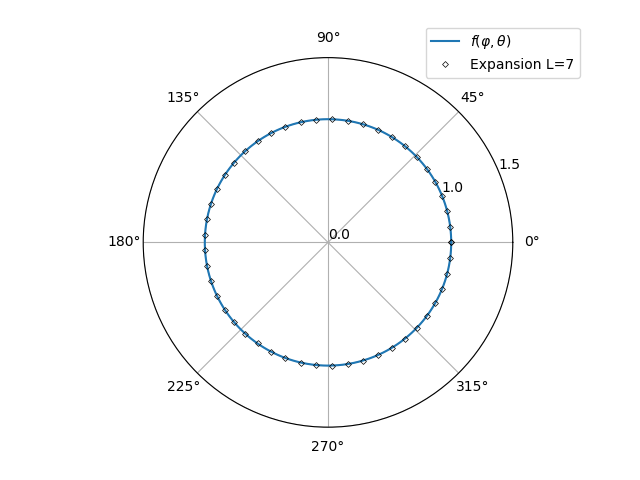
\includegraphics[width=0.8\linewidth]{Ylm_f0}
\caption{Approximation of a pure isotropic function with spherical harmonics. The plot is shown for the azimuthal angle $\varphi$ only.}
\label{fig:ylmf0}
\end{figure}

\subsubsection{Approximating an anisotropic but smooth flux}
We can construct an anisotropic function of azimuthal angle as
$$
f(\varphi,\theta) = 1+\cos (4\varphi)
$$

\begin{lstlisting}[language=python]
def F1(varphi,theta):
    return 1.0+0.1*math.cos(varphi*4)
\end{lstlisting}

Such a function requires a few more orders of spherical harmonics in order to capture the shape and, as shown in Figure \ref{fig:ylmf7}, $L=7$ closely resembles the shape. A function of this shape could appear in a fuel assembly lattice where the effective scattering and absorbtion is a strong function of azimuthal angle.

\begin{figure}[H]
\centering
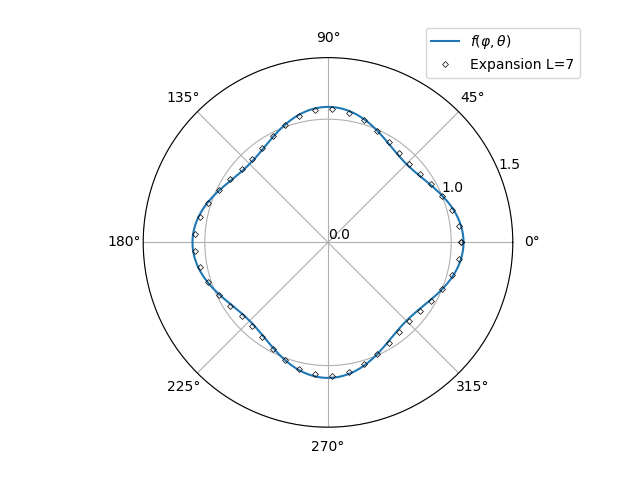
\includegraphics[width=0.8\linewidth]{Ylm_f7}
\caption{Approximation of an anisotropic smooth function with spherical harmonics. The plot is shown for the azimuthal angle $\varphi$ only. The radial dimension represents the flux magnitude.}
\label{fig:ylmf7}
\end{figure}

\newpage
\subsubsection{Approximating a directional flux (i.e. anisotropic + not-smooth)}
As a final consideration we try to construct a function that is very angular, like a beam. Such a function of angle could be
\begin{equation*}
f(\varphi,\theta) = 
\begin{cases}
\frac{2}{10} & \text{if } \quad \varphi<\frac{7}{8}\pi \\
\frac{2}{10} + \frac{6}{5}\cos (4\varphi) & \text{if }\quad \frac{7}{8}\pi \le \varphi \le \frac{9}{8}\pi\\
\frac{2}{10} & \text{if }\quad \ \varphi>\frac{9}{8}\pi \\
\end{cases}
\end{equation*}

\begin{lstlisting}[language=python]
def F2(varphi,theta):
    if (varphi<(7*math.pi/8)):
        return 0.2;
    if (varphi>(9*math.pi/8)):
        return 0.2;
    
    return 1.2*math.cos(varphi*4)+0.2
\end{lstlisting}

As expected a total number of 12 spherical harmonic orders are required to accurately represent such a directional flux (see Figure \ref{fig:ylmf12}). An additional 2D plot is shown in Figure \ref{fig:ylmf12b} which more clearly shows the oscillations of the expansion at the directions not aligned with the directional nature of the function.

\begin{figure}[H]
\centering
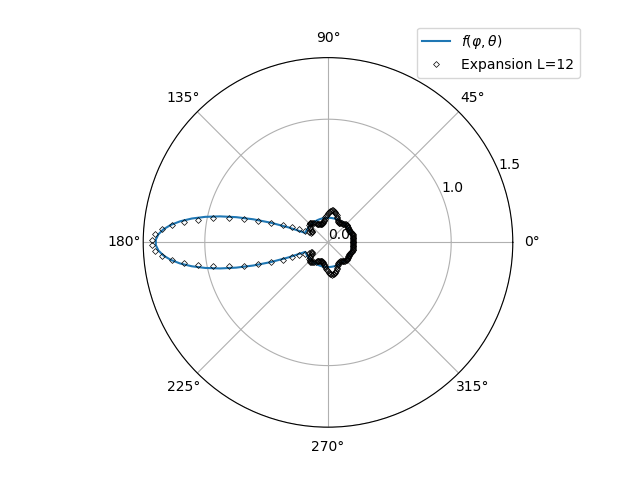
\includegraphics[width=0.8\linewidth]{Ylm_f12}
\caption{Approximation of an anisotropic smooth function with spherical harmonics. The plot is shown for the azimuthal angle $\varphi$ only. The radial dimension represents the flux magnitude.}
\label{fig:ylmf12}
\end{figure}

\begin{figure}[H]
\centering
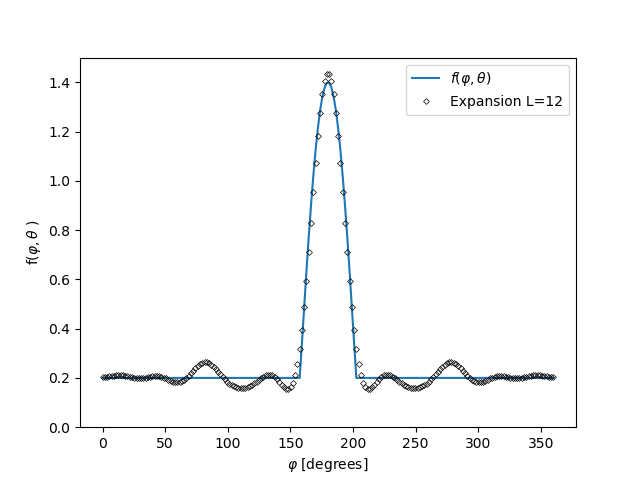
\includegraphics[width=0.8\linewidth]{Ylm_f12b}
\caption{Approximation of an anisotropic smooth function with spherical harmonics. The plot is shown for the azimuthal angle $\varphi$ only. }
\label{fig:ylmf12b}
\end{figure}

\subsection{Prototype code for real form of the spherical harmonics}
For the real form of the spherical harmonics we have a slightly modified real form 

\beqn
Y_{\ell m} (\theta, \varphi )=
\begin{cases}
 \sqrt(2)\sqrt{ \frac{(2\ell + 1)}{4\pi}   \frac{(\ell-|m|)!}{(\ell+|m|)!}}P_{\ell}^{|m|}(\cos\theta)sin\ {|m|\varphi}
& \text{if } m < 0 \\
\sqrt{ \frac{(2\ell + 1)}{4\pi}} P_{\ell}^{m}(cos\theta) & \text{if } m = 0 \\
 \sqrt(2)\sqrt{ \frac{(2\ell + 1)}{4\pi}   \frac{(\ell-m)!}{(\ell+m)!}}P_{\ell}^{m}(\cos\theta)cos\ {m\varphi}
& \text{if } m \ge 0 \\
\end{cases}
\eeqn

and the expansion coefficients are also different

\beqn 
f(\varphi,\theta) = \sum_{\ell = 0}^\infty \sum_{m=-\ell}^{\ell} f_{\ell m} Y_{\ell m}(\varphi,\theta)
\eeqn 

where
$$
f_{\ell m} = \int_{0}^{2\pi} \int_0^\pi f(\varphi,\theta)Y_{\ell m}(\varphi,\theta).sin\theta.d\theta.d\varphi
$$

for which the code is

\begin{lstlisting}[language=python]
#============================    
def Ylmcoeff(ell,m,varphi,theta):
    if (m<0):
        return math.sqrt( \
               ( (2*ell+1)/(2*math.pi) )* \
               fac(ell-abs(m))/fac(ell+abs(m)) )* \
               AssociatedLegendre(ell,abs(m),math.cos(theta))* \
               math.sin(abs(m)*varphi)
    elif (m==0):
        return math.sqrt( \
               ( (2*ell+1)/(4*math.pi) )* \
               fac(ell-m)/fac(ell+m) )* \
               AssociatedLegendre(ell,m,math.cos(theta))* \
               math.cos(m*varphi)
    else:
        return math.sqrt( \
               ( (2*ell+1)/(2*math.pi) )* \
               fac(ell-m)/fac(ell+m) )* \
               AssociatedLegendre(ell,m,math.cos(theta))* \
               math.cos(m*varphi)
\end{lstlisting}

And

\begin{lstlisting}[language=python]
def Flm(ell,m,varphi,theta):
    return F3(varphi,theta)* \
           (Legendre.Ylmcoeff(ell,m,varphi,theta))
           
#=========================== Build flm
L =12
k=-1
flm = np.zeros((L*(L+2)+1),dtype=np.complex_)
for ell in range(0,L+1):
    for m in range(-ell,ell+1):
        k=k+1
        #flm[k] = Legendre.RiemannAngLM(F1lm,ell,m)
        
        #print("l=%f, m=%f, flm=" %(ell,m), end='')
        #print(flm[k])
        flm[k] = Legendre.QuadratureIntegrateLM(Flm,GLC,ell,m)
        print("l=%f, m=%f, flm=" %(ell,m), end='')
        print(flm[k])

#============================ Build yi1
Ni1=400
varphi1=np.linspace(0,2*math.pi,Ni1)
yi1=np.zeros((Ni1))

for i in range(0,Ni1):
    yi1[i]= 0;
    v = 0
    k=-1;
    for ell in range(0,L+1):
        for m in range(-ell,ell+1):
            k=k+1
            v=v+(flm[k])* \
            (Legendre.Ylmcoeff(ell,m,varphi1[i],math.pi/2))
            yi1[i] = v
\end{lstlisting}



\newpage
\chead{References}
\begin{thebibliography}{1}
    
    
    
    
\end{thebibliography}





\end{document}